\documentclass[a4paper]{article}
\usepackage{graphicx} % Required for inserting images

\usepackage[T1]{fontenc}
\usepackage{lmodern} % Font Family
%\renewcommand{\rmdefault}{lmss}
%\renewcommand{\rmdefault}{cmss}
\renewcommand{\rmdefault}{phv}

%\usepackage[a4paper]{geometry}
\usepackage[utf8]{inputenc}
\usepackage[english]{babel}
\usepackage{newunicodechar}
\newunicodechar{δ}{\delta}

\usepackage{graphicx, setspace}
\usepackage{setspace}
% Using \doublespacing in the preamble 
% changes text to double line spacing

\usepackage{pgfgantt}
\usepackage{pgfcalendar}
\usepackage{adjustbox}
\usepackage[dvipsnames]{xcolor}
\usepackage[toc,page]{appendix}
\usepackage{subcaption}

\usepackage{graphicx}
\usepackage{eso-pic}

\usepackage[backend=biber,style=numeric,sorting=none]{biblatex}
%\bibliographystyle{unsrt}
\addbibresource{mybib.bib}
%\usepackage{biblatex} %Imports biblatex package
%\addbibresource{mybib.bib} %Import the bibliography file

\usepackage[all]{background}
\usepackage{lipsum}
\SetBgContents{ \color{black!60} \texttt{{\scriptsize {\it Preliminar 24.03.2026v1.0} }} }% Set contents
\SetBgPosition{-0.5cm,-5.0cm}% Select location
\SetBgOpacity{1.0}% Select opacity
\SetBgAngle{90.0}% Select rotation of logo
\SetBgScale{2.0}% Select scale factor of logo

\usepackage{overpic}
\usepackage{xcolor} 
\usepackage{soul}
\usepackage{enumitem}

%#######################################################################
\usepackage[a4paper,
            bindingoffset=10pt,
            left=3.0cm,
            right=3.0cm,
            top=1.0cm,
            bottom=2.5cm,
            headheight=1.25cm,
            headsep=0.9cm,
            footskip=1.5cm,
            includehead,
            includefoot
            ]{geometry}
%Set header and footer using the fancyhdr package

\usepackage{fancyhdr}
\pagestyle{fancy}
\fancyhf{}

\lhead{
\includegraphics[height=1.75cm,angle=270,trim= 9cm 2.35cm 9cm 24.65cm, clip]{Figures/lnls_logo.pdf}} % left logo
\rhead{
\includegraphics[height=3.25cm,angle=270,trim= 9.25cm 7.5cm 9.25cm 14.5cm, clip]{Figures/lnls_logo.pdf}} % right logo
\rfoot{
\includegraphics[height=4.5cm,angle=270,trim= 9.cm 15cm 9.cm 2.25cm, clip]{Figures/lnls_logo.pdf}}
\cfoot{\thepage}

\renewcommand{\headrulewidth}{0pt} % remove rule below header

\pdfpkresolution=300

%#######################################################################

\begin{document}

\pagenumbering{gobble}
\begin{titlepage}

\AddToShipoutPictureBG*{%
    \AtPageLowerLeft{%
        %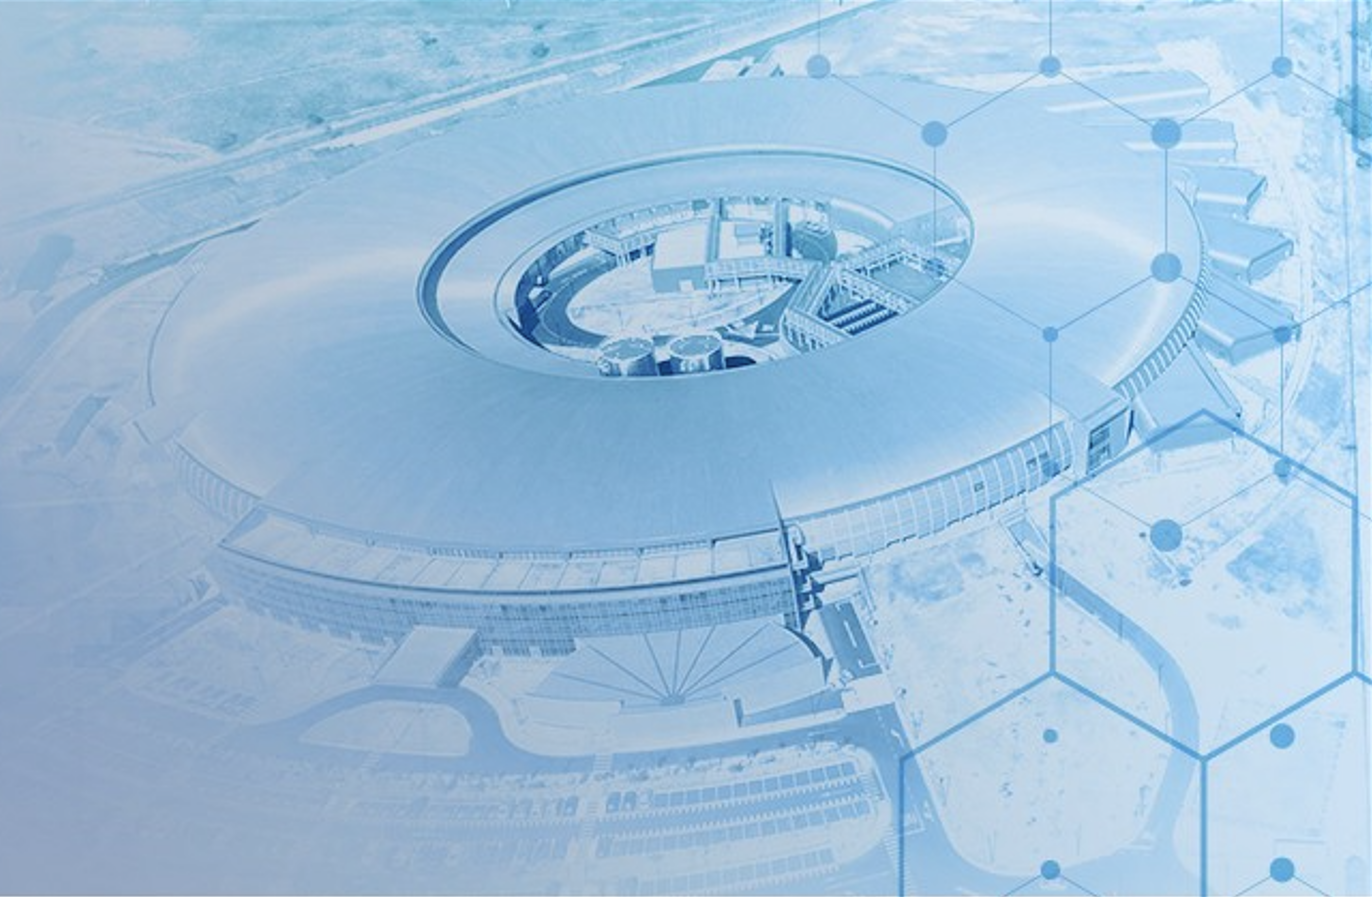
\includegraphics[width=\paperwidth, height=\paperheight, trim= 2cm 0.cm 2cm 0cm, clip]{frontpage/cnpem_cover.PNG}%
        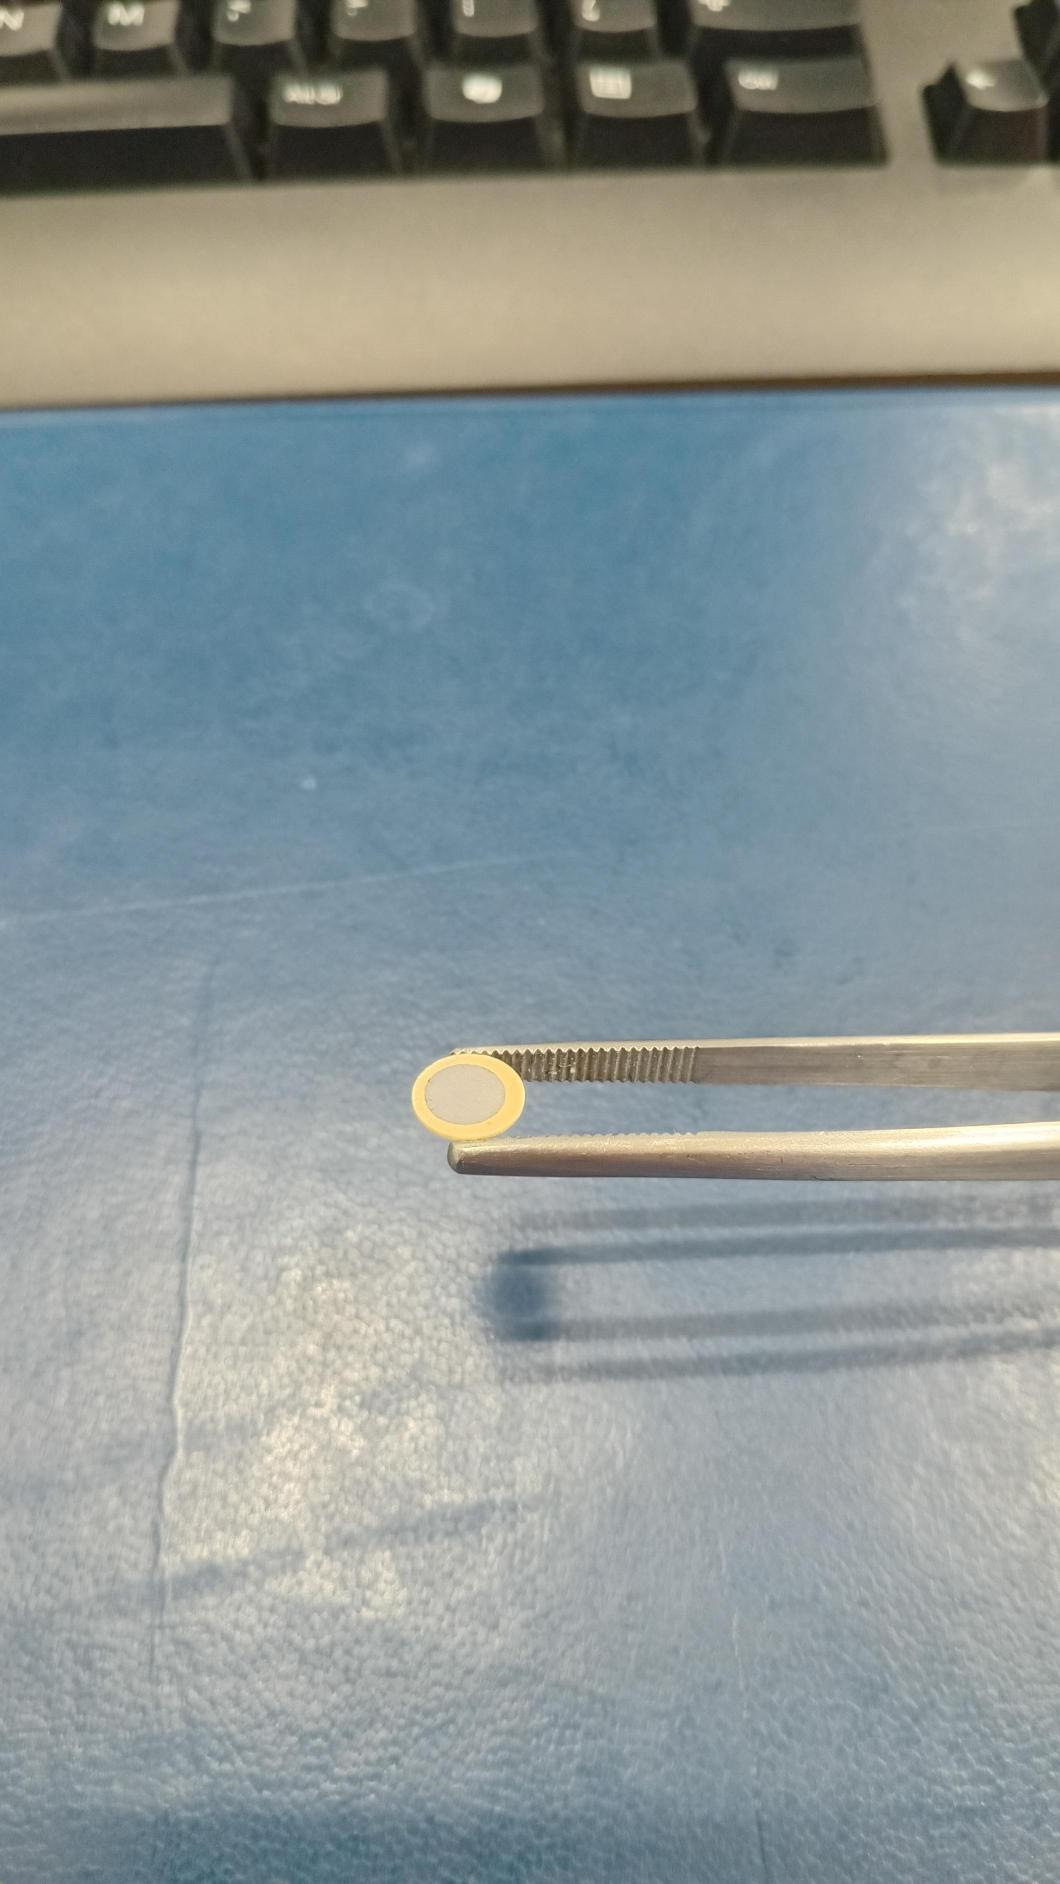
\includegraphics[width=\paperwidth, angle=0, height=\paperheight, trim= 0cm 2.cm 2cm 11.5cm, clip]{frontpage/cover.PNG}%
    }%
}

{\centering
{
\includegraphics[height=8.25cm,angle=270,trim= 9.25cm 7.5cm 9.25cm 14.5cm, clip]{Figures/lnls_logo.pdf}}

\vspace{4.5cm}

\textbf{\color{black} \huge Innovative Cells for in-situ and operando studies of SOFC/SOEC and steam reforming of ethanol}
\vspace{3cm}


\vspace{0.5cm}


\vspace{0.5cm}


\vspace{3.5cm}

\texttt{\huge Autor: Renato Aparecido Negrão de Oliveira}
\vspace{1.cm}

\texttt{\huge Autor: Santiago José Alejandro Figueroa (CNPEM)}
\vspace{1.25cm}

Campinas,
\vspace{0cm}

2026

\pagestyle{empty}
}
\end{titlepage}

%\doublespacing
\SetSinglespace{1.5}
\singlespacing

\tableofcontents

\pagenumbering{arabic}
%\include{Introduction}
\include{ProjectSummary}
%###########################################################
%#
%#
%#
%###########################################################
\section{Research Project}

Fuel cells are electrochemical energy conversion devices that directly transform chemical energy into electrical energy without the need for combustion processes, making them essential technologies for the global energy transition toward sustainable power generation systems \cite{Nigel2017}. Unlike conventional thermal devices, fuel cells rely on electrochemical reactions occurring at electrodes separated by an ion-conducting electrolyte, enabling high efficiency and low environmental impact \cite{Gurbinder2016}.

Fuel cells convert chemical energy directly into electrical energy through a redox reaction. Like thermal devices, they operate continuously as long as fuel and oxidant are supplied. Because of this nature, fuel cells are capable of continuously producing electricity with high conversion efficiency.

Several types of fuel cell technologies exist, each defined primarily by the electrolyte material and operating temperature range \cite{Gurbinder2016,skinnerd:2008}. Examples include polymer electrolyte membrane fuel cells, alkaline fuel cells, and solid oxide fuel cells. Despite differences in materials and temperature regimes, all fuel cell technologies share common characteristics such as high energy conversion efficiency, absence of moving mechanical parts, modular scalability, and low or near-zero pollutant emissions during operation.

Applications of fuel cells extend to a wide technological spectrum, from portable electronic devices and backup power systems to transportation and large-scale distributed electricity generation \cite{BinZhu2020}. These technologies contribute to reducing dependence on fossil fuels, lowering greenhouse gas emissions, improving energy security, and supporting the development of a hydrogen-based energy infrastructure.

Growing global concern regarding energy security, atmospheric pollution and greenhouse gas emissions has intensified research into environmentally sustainable energy technologies. Among the various fuel cell systems, Solid Oxide Fuel Cells (SOFC) have attracted considerable scientific and technological interest due to their high efficiency, fuel flexibility, and long-term stability \cite{Kevin2003}. SOFCs can operate using hydrogen, carbon monoxide, methane, and other hydrocarbon-based fuels, reducing the need for highly purified hydrogen and enabling integration with existing fuel infrastructures.

The project focuses on  symmetric Intermediate-Temperature Solid Oxide Fuel Cells \cite{JuanCarlos2011,KejunZhu2022,Muhammad2022,Liliana2016}, which operate typically between 500 and 700°C. Operating in this temperature range reduces thermal degradation, expands material choices, and lowers system costs while maintaining sufficient ionic conductivity and catalytic activity. Because of their symmetric configuration and reversible electrochemical behavior, these devices can also function as Solid Oxide Electrolyzer Cells (SOEC), enabling efficient electrolysis of water \cite{Meng2008}. When powered by renewable electricity, SOEC systems can produce green hydrogen, a key energy carrier in decarbonized energy systems.

As shown in Figure \ref{sofc}, a Solid Oxide Fuel Cell device is composed of a cathode, an anode, and a dense ceramic electrolyte. At the cathode, oxygen reduction reactions (ORR) convert molecular oxygen into oxide ions. Perovskite oxides such as lanthanum strontium manganite exhibit excellent electrocatalytic performance for this reaction \cite{Sacanell2017,Diego2017,JACOBSON2012478}. The anode promotes fuel oxidation (or Hydrogen Oxidation Reaction, HOR), commonly employing nickel yttria stabilized zirconia cermets capable of hydrogen oxidation and internal reforming of methane-containing fuels \cite{Nigel2017,skinnerd:2008}. The electrolyte is typically a dense yttria-stabilized zirconia ceramics, which provides high oxide-ion conductivity and chemical stability at elevated temperatures \cite{Nigel2017,skinnerd:2008}.

\begin{figure}[h]
\centering
    \begin{overpic}[width=.75\linewidth,keepaspectratio,angle=0,trim=0.cm 0.cm 0.cm 0.cm, clip]{Figures/SOFC.png}
    \put(45,85){\Large \bf \textcolor{Blue}{Cathode}}
    \put(62,60){\Large \bf \textcolor{Black!90}{Electrolyte}}
    \put(-3,55){\Large \bf \textcolor{Orange}{Anode}}

    \put(30,75){\Large \bf \textcolor{White}{1/2O$_2$+2e$^-$ $\to$ 2O$^{2-}$ }}
    
    \put(41,63,55){\Large \bf \textcolor{Black}{ $\downarrow$ }}
    \put(45,62.5){\Large \bf \textcolor{Black}{ O$^{2-}$ }}
    
    \put(30,35){\Large \bf \textcolor{White}{H$_2$+O$^{2-}$ $\to$ H$_2$O+2e$^-$}}
    
    \end{overpic}
    
    \caption{SOFC device scheme showing the Cathode Oxygen Reduction Reaction (ORR), and the Anode Hydrogen Oxidation Reaction (HOR). The ionic conductivity ($\sigma_{ion}$) of the electrolyte is governed by the migration of oxygen vacancies ($V_O ^{\cdot\cdot}$) in the crystal lattice, which follows the Arrhenius law dependence on temperature \cite{Nigel2017}. Figure addapted from \cite{HU2023}. }
    
    \label{sofc}
\end{figure}


A major limitation of conventional SOFC technology is that peak efficiency occurs at temperatures near 900–1000$^\circ$C \cite{Nigel2017,Gurbinder2016,skinnerd:2008}. Such high temperatures restrict material selection for interconnects and structural components and accelerate degradation mechanisms such as thermal expansion mismatch, phase instability, and chemical inter diffusion. And materials such as lanthanum, strontium, and chromium are often required, which are costly. These challenges have motivated extensive research into materials capable of efficient operation at intermediate temperatures.

Despite significant advances in intermediate-temperature SOFC materials, several \linebreak state-of-the-art cathode materials rely on elements such as lanthanum, cobalt, and cerium, which present economic, and environmental concerns. This project proposes the exploration of alternative mixed ionic-electronic conductors based on more abundant and lower-cost elements such as iron and molybdenum. Candidate materials include perovskite-structured compounds such as (La,Sr)(Fe,Mo)O$_{3-\delta}$, (Ba,Sr)(Fe,Mo)O$_{3-\delta}$, (La,Sm)(Fe)O$_{3-\delta}$, and  (La,Sm)(Fe,Mo)O$_{3-\delta}$. These materials have shown promising electrochemical behavior in related studies \cite{GIL2024,MEJIAGOMEZ2020} and may provide competitive catalytic performance while reducing cost and environmental impact.

\hl{Would we like to expand the set of candidate materials for SOFC applications and provide technical justification for their inclusion?}\dotfill

\dotfill

\dotfill

\dotfill

\dotfill

In parallel, Solid Oxide Electrolyzer Cell (SOEC) systems will be developed using cobalt-free oxygen electrode materials based on (Ln,Sr)Fe$_{0.8}$Cu$_{0.2}$O$_{3-\delta}$ perovskite oxides, where Ln represents lanthanide elements such as La, Nd, Pr, or Gd. Among these, LaSFCu compositions have demonstrated excellent reversible performance in SOFC/SOEC operation. Composite materials incorporating ceria-based fluorites, such as LSFCu-CeO$_2$ nanocomposites with ceria contents, will also be investigated due to their enhanced oxygen transport and catalytic activity \cite{Natasha2026}.

\hl{Would we like to expand the set of candidate materials for SOEC applications and provide technical justification for their inclusion?}\dotfill

\dotfill

\dotfill

\dotfill

\dotfill

Another topic proposed in this project is the valuation and development of nano catalysts materials for the steam reforming of ethanol (SRE). Bio-ethanol energy is a renewable energy resource, and its utilization can reduce pollution \cite{FENG2023}.  Bio-ethanol can be obtained from the fermentation of various raw materials containing sucrose, and cellulosic biomass \cite{Tripodi2018}. It also has high hydrogen content, non-toxicity, easy storage, and processing. Therefore, producing hydrogen from ethanol reforming process has gained widespread attention. The ethanol reforming process can be achieved by different oxidants \cite{FENG2023} including H$_2$O for the process called steam reforming of ethanol. 

Commonly used SRE catalysts are supported catalysts with active group VIII metals and Cu, supported by thermostable oxide ceramics such as CeO$_2$, Al$_2$O$_3$, SiO$_2$ ZrO$_2$, etc. Considering the results from previous publications by the group \cite{}, we will work on the design of novel nano-structured Ni-Cu bimetallic materials as catalysts for steam reforming of ethanol and will adjust their composition and morphology to optimize reactivity and selectivity for this reaction.

\hl{Would we like to expand the set of candidate materials for SRE applications and provide technical justification for their inclusion?}\dotfill

\dotfill

\dotfill

\dotfill

\dotfill

The synthesized materials will undergo comprehensive characterization to determine structural, morphological, and redox properties. Techniques will include X-ray diffraction, and electron microscopy. Catalytic and electrocatalytic behavior will be evaluated using gas chromatography under controlled reaction conditions. These laboratory measurements will be performed at the CNPEM support facilities and will be complemented by in-situ and operando synchrotron based X-ray absorption spectroscopy experiments to directly observe structural and electronic changes during operation.

The research group possesses strong expertise in nanomaterial synthesis and preparation using multiple processing routes, including sol-gel synthesis, and combustion methods \cite{Diego2011,Lucia2016,Diego2024}. Those expertise ensures the feasibility of producing high-quality materials and overcoming synthesis challenges associated with complex perovskite systems and nanocomposite electrodes.

A central component of this project is the development of specialized experimental instrumentation compatible with synchrotron characterization. The project will leverage the capabilities of the QUATI beamline for nanoscale investigation of functional materials \cite{Santiago2023}. The methodology involves experimental engineering cells capable of operating under realistic catalytic and electrochemical conditions while allowing X-ray transmission and precise environmental control. These measurement cells will enable direct observation of catalytic reactions, electrocatalytic processes, and ionic transport phenomena in nanostructured materials during operation, establishing a powerful experimental framework for understanding and optimizing next-generation solid oxide electrochemical technologies.

\hl{Include also Time Differential Perturbed Angular Correlation technique for material characterization}\dotfill

\dotfill

\dotfill

\dotfill

\dotfill

Finally, the integration of advanced materials development techniques, catalytic hydrogen production via steam reforming of ethanol, and operando synchrotron characterization represents a comprehensive approach to addressing key scientific and technological challenges in electrochemical energy conversion systems, and will be the focus of this proposal.

\section{Methodology}

%\subsection{Quati beamline}

The development of advanced catalytic and electrochemical materials for sustainable energy conversion requires analytical methodologies capable of resolving structural, electronic, and chemical transformations under realistic operating conditions. In this context, the integration of synchrotron radiation techniques with purpose-designed experimental cells represents a step toward understanding and controlling complex physico-chemical processes. 

The QUATI (Quick X-Ray Absorption Spectroscopy for Time and Space Resolved Experiments) beamline at the Brazilian fourth-generation synchrotron light source Sirius provides an unique platform for such investigations \cite{Santiago2023}. Operated by the Laboratório Nacional de Luz Síncrotron within the Centro Nacional de Pesquisa em Energia e Materiais, Sirius delivers high brilliance and low emittance X-ray beams that enable advanced spectroscopic measurements with unprecedented temporal and spatial resolution. As shown in Figure \ref{quati}, the QUATI beamline is specifically designed for high-resolution X-ray absorption spectroscopy, and offers capabilities ideally suited for in-situ and operando investigations of catalytic systems for steam reforming of ethanol and electrochemical devices such as solid oxide fuel cells and solid oxide electrolysis cells.

X-ray absorption spectroscopy provides element-specific information on local atomic structure and configuration without requiring long-range order. The technique encompasses the near-edge region, known as X-ray absorption near edge structure (XANES), which is sensitive to oxidation state and coordination symmetry \cite{XU2024}, and the extended region, known as extended X-ray absorption fine structure (EXAFS), which yields quantitative information on interatomic distances, coordination numbers, and disorder parameters \cite{MALZER2021}. 

\begin{figure}[h]
    \centering
    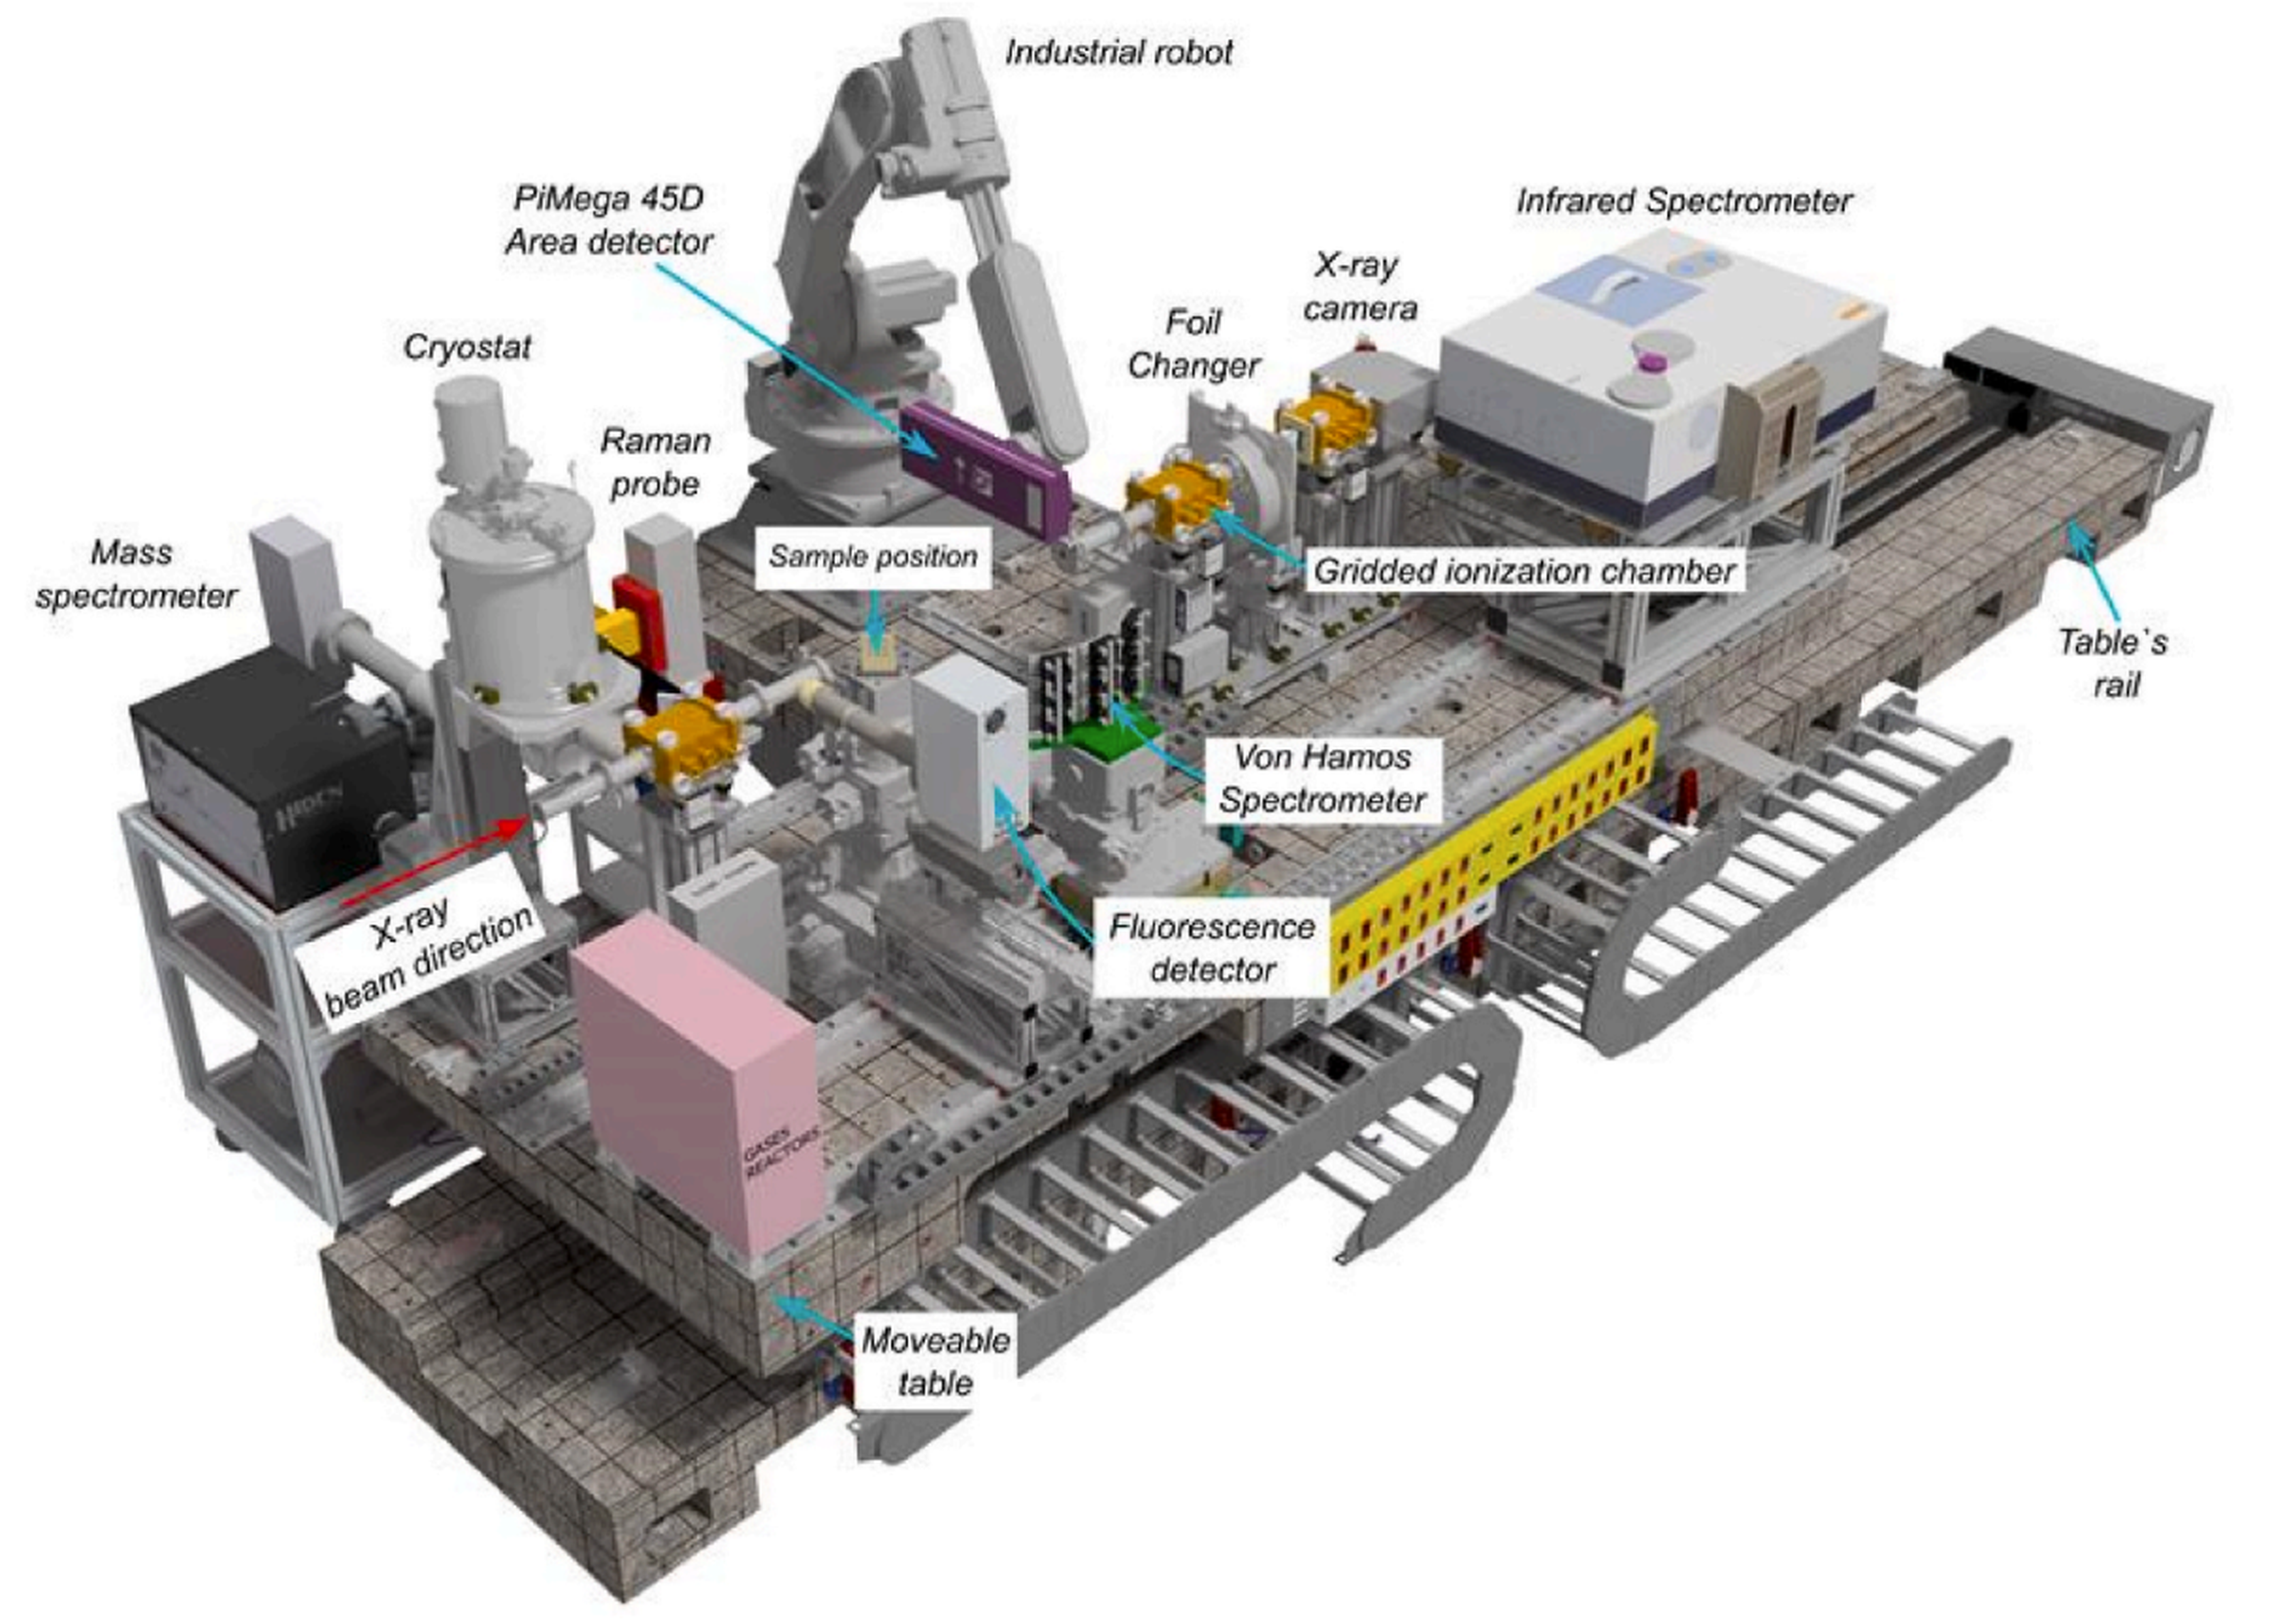
\includegraphics[width=.8\linewidth]{Figures/QUATI.png}
    \caption{Quati experimental beamline and subsystems. Figure reproduced from \cite{Santiago2023}.}
    \label{quati}
\end{figure}

The QUATI beamline has been designed to exploit the high brilliance of Sirius to perform rapid energy scans, enabling time-resolved XANES and EXAFS measurements on the millisecond to second timescale \cite{Santiago2023}. Such temporal resolution is critical for tracking redox oscillations, phase transitions, and active site changes during catalytic reactions and electrochemical processes.

The energy range of QUATI, extending from approximately 4.5 keV to 35 keV allows access to K edges of {\it 3d} transition metals and heavier elements, as well as the L edges of heavy elements. This spectral coverage is particularly relevant for materials based on nickel, cobalt, iron, copper, strontium, zirconium, yttrium, platinum, palladium, lanthanum, cerium, and gadolinium which are frequently employed in steam reforming of ethanol and solid oxide electrochemical devices.

In addition, the integration of innovative in-situ and operando electrochemical cells with QUATI spectroscopic capabilities is central to advancing the understanding of catalytic processes. These cells must fulfill several requirements. They must allow operation at high temperatures, often exceeding 800$^\circ$C for steam reforming and solid oxide electrochemical devices. They must withstand controlled gas atmospheres containing steam, ethanol, hydrogen, and oxygen. They must provide uniform temperature distribution, minimize X-ray absorption by cell components, and permit simultaneous complementary measurements such as electrochemical impedance spectroscopy (EIS). Furthermore, the cells must be designed to accommodate the beam path and scanning modes of the beamline, ensuring optimal signal-to-noise ratio and reproducibility.

For solid oxide fuel cells under operating conditions, the electrodes experience large oxygen chemical potential gradients \cite{Takashi2017}, thermal stress, and redox cycling. The local electronic structure of transition metal in these electrodes directly influences catalytic activity for oxygen reduction (ORR) and fuel oxidation reactions (HOR) \cite{Takashi2017,CHENG2023}. Operando XANES measurements at the Co, Fe, or Ni K edges allow quantification of valence state changes as a function of applied current density and gas composition. By integrating a custom-designed electrochemical cell compatible with high-temperature operation and X-ray fluorescence geometry \cite{Seval2021,Yoichiro2020}, one can measure the X-ray spectrum while the device is generating power.

The design of innovative electrochemical cells for synchrotron experiments requires optimization. The cell must maintain gas-tight separation between fuel and oxidant compartments while allowing X-ray photons to reach the electrode regions. Electrical contacts must withstand high temperatures without introducing significant X-ray absorption or scattering artifacts, and the geometry must ensure that the X-ray beam probes a representative volume of the electrode with minimal background contributions. At QUATI, the possibility of quick scanning enables the acquisition of sequential spectra during dynamic changes. This capability allows the correlation of structural changes with electrochemical performance in real time, offering insight into degradation mechanisms such as segregation, phase transition, or interfacial reactions \cite{Yao2019}.

For solid oxide electrolysis cells, operating in reverse mode to produce hydrogen, the scenario shares similar challenges and also similar operating conditions. For instance, operando XAS at the K or L edge under electrolysis conditions can quantify small shifts in edge position indicating changes in electronic structure associated with the processes \cite{Skinner2013}. Additionally, Time-resolved EXAFS can provide information on variations of the chemical bond length associated with oxygen non-stoichiometry changes during operation. By coupling these spectroscopic observations with electrochemical impedance data, it will become possible to distinguish between bulk and interfacial degradation pathways.

As illustrated in Figure \ref{methodology}, the research methodology enabled by QUATI in combination with in-situ cells extends beyond the empirical observation. The high resolution XANES and EXAFS data obtained under realistic conditions can be combined with density functional theory calculations to construct accurate structural models of catalytically active sites \cite{XU2024,Lucchetti2024}. By fitting experimental spectra with theoretically generated simulations, it will be possible to determine such structural information, guiding the selection of dopants, support compositions, and synthesis routes.

\begin{figure}[h]
    \centering
    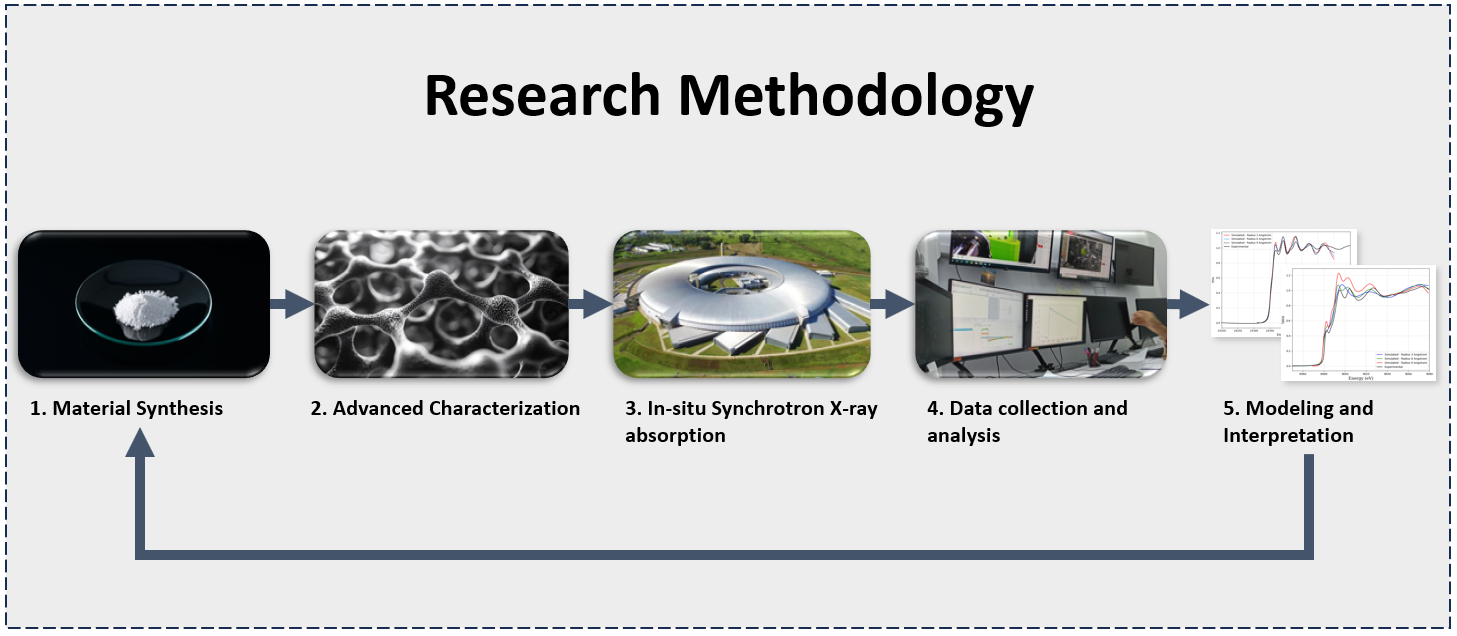
\includegraphics[width=1.\linewidth]{Figures/methodology.PNG}
    \caption{Figure showing a diagram illustrating the research methodology.}
    \label{methodology}
\end{figure}

The successful implementation of these research programs depends on the rigorous engineering of experimental infrastructure. Gas systems must deliver precisely controlled mixtures, temperature control must be accurate within a few degrees to avoid combination of thermal effects with intrinsic chemical changes. Data acquisition systems must synchronize X-ray scanning with external triggers to capture fast processes. Advanced data analysis pipelines, including principal component analysis, are required to deconvolute overlapping spectral features and identify distinct chemical species. The high photon flux at Sirius ensures that high signal-to-noise ratios can be achieved even under demanding conditions, enabling quantitative interpretation from the experiments.

%##########################
%\hl{START MODIFICATION}

Perturbed Angular Correlation Spectroscopy (PAC) will be employed to probe the local atomic and electronic environment of SOFC materials through hyperfine interactions, namely the magnetic hyperfine field (MHF) and electric field gradient (EFG), providing insights into crystal structure, defects, and local symmetry.

Experiments will be conducted at the Laboratory of Hyperfine Interactions (LIH) at IPEN (Brazil), which benefits from access to the IEA-R1 reactor for the production of radioactive probe nuclei (e.g., $^{111}$In, $^{181}$Hf). For this project, a newly implemented digital PAC spectrometer (figure \ref{pac}), based on LaBr$_3$ detectors and a CAEN acquisition system, will be used. This setup offers improved time resolution, higher counting efficiency, and faster data acquisition compared to conventional analog systems, allowing simultaneous analysis of multiple decay cascades and enhanced statistical reliability.

\begin{figure}[h]
    \centering
    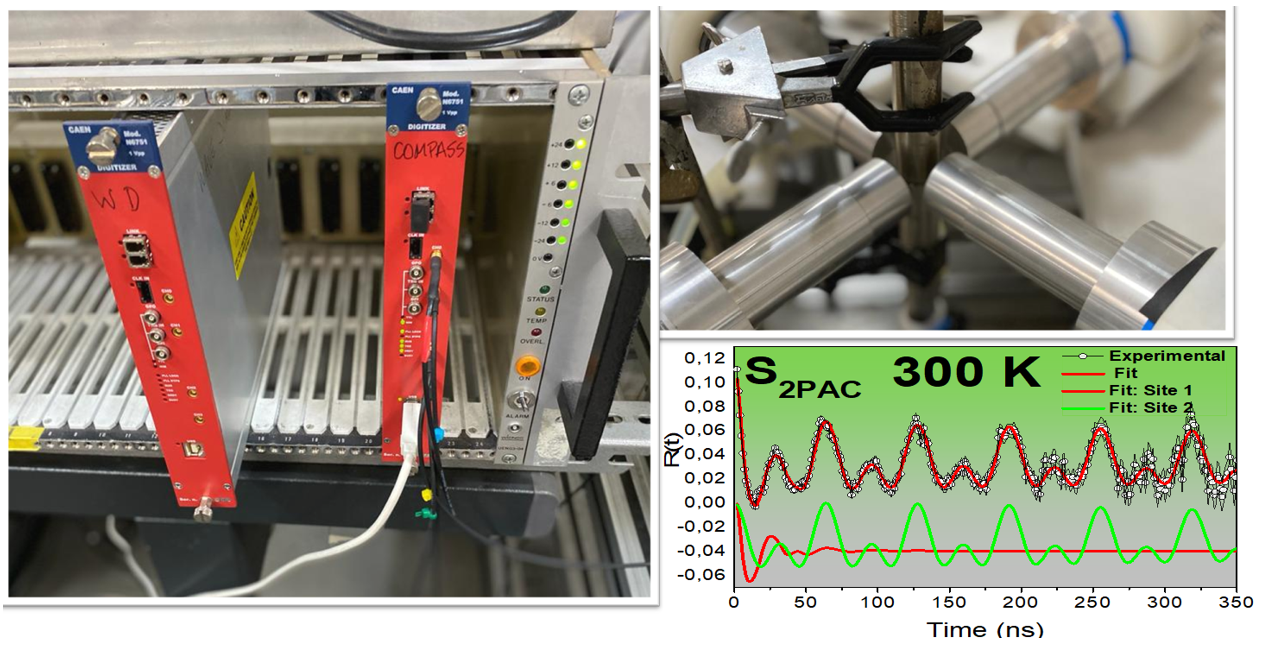
\includegraphics[width=1.\linewidth]{Figures/PAC.PNG}
    \caption{(a) Digital PAC spectrometer at LIH-IPEN; (b) furnace coupled to the digital spectrometer; and (c) characteristic PAC spectra of  $^{111}$In probe nuclei in a Ni-based catalyst.}
    \label{pac}
\end{figure}

Additionally, a dedicated high-temperature furnace enables in situ PAC measurements under controlled atmospheres, simulating realistic SOFC operating conditions. This capability allows the investigation of temperature-dependent phenomena such as defect dynamics, oxygen vacancy behavior, and phase stability, providing a comprehensive understanding of structure–property relationships under operando conditions.


%\hl{END MODIFICATION}
%##########################

In summary, the convergence of high-brilliance synchrotron radiation at Sirius, advanced X-ray absorption spectroscopy at the QUATI beamline, and purpose built innovative in-situ and operando cells establishes a framework for investigating catalytic materials for ethanol steam reforming and solid oxide electrochemical devices. The ability to probe local atomic structure and electronic configuration under realistic conditions, with high temporal and spatial resolution, addresses a longstanding gap in catalysis and electrochemistry research. Through rigorous integration of spectroscopic analysis, and theoretical modeling, this approach enables the development of next-generation materials with improved activity, stability, and sustainability. The scientific and technological implications extend from fundamental understanding of the chemical reaction dynamics to practical deployment of renewable energy systems, positioning this research at the forefront of advanced energy materials science.
\section{Expected Results}

The understanding of material behavior under realistic operating conditions is essential for advancing catalytic and electrochemical energy conversion technologies. In systems such as SOFC/SOEC cells, and catalytic reactors for steam reforming of ethanol (SRE), the working principles are governed by mechanisms involving surface catalysis, electrocatalytic charge transfer, defect chemistry, and ionic and electronic transport in complex oxides. These processes are highly sensitive to temperature, gas composition, and electrochemical processes. And they frequently induce dynamic structural and electronic changes that cannot be captured by ex-situ characterization. To address this challenge, the present project emphasizes the development of advanced instrumentation based on synchrotron techniques capable of probing materials in-situ and operando.

The experimental strategy will be implemented at CNPEM using the fourth-generation synchrotron light source Sirius. In particular, the QUATI beamline will be employed due to its capability for in-situ and operando material characterization. The high brilliance, stability, and energy tunability of the source enable high-resolution X-ray absorption spectroscopy, providing element-specific information on oxidation state, coordination environment, and local atomic structure under realistic reaction conditions. Custom-designed high-temperature electrochemical and catalytic cells will be integrated into the beamline environment, allowing measurements under controlled gas atmospheres and applied electrical bias. This approach ensures that catalytic, electrocatalytic, and transport mechanisms are measured while the material is in working conditions, thereby establishing direct correlations between atomic-scale dynamics and macroscopic performance.

These experiments are crucial for elucidating degradation mechanisms that limit device durability. Materials employed in SOFC/SOEC devices and ethanol reforming catalysts are subjected to redox cycling, high thermal loads, chemical gradients, and reactive intermediates that promote phase segregation, ion migration, carbon deposition, and microstructural degradation. Operando X-ray absorption spectroscopy, combined with electrochemical measurements, enables early detection of such phenomena by monitoring changes in electronic structure, local bonding, and electro-catalytic efficiency. 

The results will significantly advance the understanding of the processes, and support the optimization of compositions, microstructures, and operating conditions. Most importantly, the advanced instrumentation and standardized experimental setups developed within this project will be made available to the LNLS user community, expanding the analytical capabilities for a broad range of electrochemical devices and catalytic systems and fostering collaborative research across disciplines.

In summary, we expect to achieve significant results in the following areas; the development and optimization of new nano materials for SOFCs and SOECs. These materials are intended to be cost-effective and durable, thereby contributing to efficient energy generation and hydrogen production; the development and optimization of new catalysts for the steam reforming of ethanol, which is particularly important for enhancing the ethanol potential and deliver economic benefits; and the engineering of specialized, innovative cells for in-situ and operando investigations of solid oxide cells and catalytic processes.

\section{Project timeline}

The project timeline is organized into five phases reflecting the complexities of a material research program progressing from synthesis to operando validation and scientific dissemination. 

Phase I — Materials Development: The project begins with the synthesis of nanostructured materials for solid oxide fuel cells (SOFCs), solid oxide electrolyzer cells (SOECs), and nanocatalysts for ethanol steam reforming. The overlap during the initial quarters allows rapid iteration between compositions, microstructure control, and defect engineering strategies. In parallel, the conceptual design of specialized in-situ and operando cells for experiments at the QUATI beamline is undertaken, ensuring that material design is aligned from the start with synchrotron compatibility requirements such as X-ray transparency, thermal stability, and controlled gas atmosphere operation.

Phase II — Advanced Characterization: During the second stage of the timeline, characterization of all developed nanomaterials becomes central. Crystallographic analysis, phase stability assessment, and lattice parameter refinement are performed to confirm phase purity. Simultaneously, textural and morphological characterization provides insight into porosity distribution, and particle size evolution. This phase will guide the selection of candidate materials. Electrochemical and redox catalytic characterizations are introduced at this point, allowing evaluation of polarization resistance, catalytic efficiency, and redox stability under controlled laboratory conditions. The overlap of synthesis refinement with characterization ensures rapid feedback and optimization.

Phase III — Device Integration: The assembly of small-sized SOFCs and SOECs marks the transition from material evaluation to device validation. These prototype cells serve as platforms for electrochemical benchmarking and degradation studies. In parallel, optimization of the QUATI beamline and PAC spectroscopy configuration for in-situ and operando studies is initiated. Initial in-situ experiments validate experimental geometry, signal-to-noise ratios, and operability under realistic redox and reforming environments.

Phase IV — In-Situ/Operando Infrastructure and Experiments: Fine-tuning of analytical programs for X-ray absorption spectroscopy ensures the extraction of oxidation states, coordination numbers, and dynamic structural evolution. This evaluation phase is essential to identify active phases, degradation pathways, and structural changes.

Phase V — Modeling, Data Analysis and Publications: Comprehensive analysis of in-situ/operando results consolidates the interpretation of catalytic and electrochemical behavior. This stage integrates electrochemical data, structural evolution, and X-ray absorption spectroscopy data into a unified framework. The final quarters are dedicated to scientific dissemination, during which the findings are structured into publications.

As explained, the project timeline covers eight quarters (24 months), as shown in the Figure \ref{projecttimeline}, and progresses from synthesis to device operando validation, with mechanisms that maximize feedback between materials development and advanced characterization. This minimizes risk, and accelerates optimization.

\begin{figure}[h]
\begin{spacing}{0.8} 
 
\begin{ganttchart}[
   hgrid={*7{gray, dotted}},
   vgrid={*5{gray, dotted}}, 
   x unit=1.15cm,
   y unit chart=1.0cm,
   time slot format=isodate,
   title label font=\color{white},
   title/.style={fill=black!60, draw=none},
   time slot unit=month,
   bar label node/.append style={align=left,text width=0.4\textwidth},
   bar/.append style={draw=none, fill=Turquoise},
   bar incomplete/.append style={fill=black!60}, 
   vrule/.style={dashed,teal},%BrickRed
   ]{2025-01-01}{2025-08-01}
    %\gantttitlecalendar{year} \\
    \gantttitlelist{1,...,8}{1}\\
    %content bars

    % ---- Synthesis ---
    \ganttbar{{\small \color{black!60} 1- Synthesis of nano materials for Fuel Cells SOFCs}}{2025-01-01}{2025-02-01}
    \ganttbar{}{2025-06-01}{2025-06-01}\\
    % ---- Synthesis ---
    \ganttbar{{\small \color{black!60} 2- Synthesis of nano materials for Electrolyzers SOECs}}{2025-01-01}{2025-02-01}
    \ganttbar{}{2025-06-01}{2025-06-01}\\
    % ---- Synthesis ---
    \ganttbar{{\small \color{black!60} 3- Synthesis of Nanocatalysts for Steam Reforming of Ethanol}}{2025-01-01}{2025-02-01}
    \ganttbar{}{2025-06-01}{2025-06-01}\\

    % ---- Structural ----
    \ganttbar{{\small \color{black!60} 4- Structural Characterization of All Developed Nanomaterials}}{2025-02-01}{2025-03-01}\\
    % ---- Textural ----
    \ganttbar{{\small \color{black!60} 5- Textural, and Morphological Characterization of All Developed Nanomaterials }}{2025-02-01}{2025-03-01}\\
    % ---- Electrochemical ----
    \ganttbar{{\small \color{black!60} 6- Electrochemical Characterization of Nanomaterials for SOFCs and SOECs}}{2025-02-01}{2025-03-01}
    \ganttbar{}{2025-07-01}{2025-08-01}\\
    % ---- Redox/Catalytic ----
    \ganttbar{{\small\color{black!60} 7- Redox and Catalytic Characterization of All Proposed Nanomaterials}}{2025-03-01}{2025-03-01}
    \ganttbar{}{2025-07-01}{2025-07-01}\\
   
    % ---- Cell Assembly ----
    \ganttbar{{\small \color{black!60} 8- Assembly of Small-Sized SOFCs and SOECs for Testing}}{2025-03-01}{2025-03-01}\\
    
    
    % ---- In-situ Design ----
    \ganttbar{{\small \color{black!60} 9- Design of Cells for In-Situ/Operando Experiments on QUATI Beamline}}{2025-01-01}{2025-02-01}\\
    % ---- Beamline Optimization ----
    \ganttbar{{\small  \color{black!60}  10- Optimization of QUATI Beamline and PAC spectroscopy for In-Situ/Operando Studies}}{2025-04-01}{2025-04-01}\\
    % ---- Cell Construction ----
    \ganttbar{{\small  \color{black!60} 11- Construction of Reaction Cells for In-Situ/Operando Experiments on QUATI Beamline and PAC spectroscopy}}{2025-03-01}{2025-04-01}\\
    % ---- Initial Operando ----
    \ganttbar{{\small  \color{black!60}  12- Initial In-Situ/Operando Experiments on QUATI Beamline}}{2025-04-01}{2025-04-01}\\
    % ---- Data Programs ----
    \ganttbar{{\small  \color{black!60}  13- Fine-Tuning of Programs for Analysis of In-Situ/Operando Experimental Data}}{2025-04-01}{2025-06-01}\\
    % ---- Modeling ----
    \ganttbar{{\small  \color{black!60}  14- Evaluation of All Developed Materials through In-Situ and Operando Experiments}}{2025-04-01}{2025-07-01}\\
    % ---- Data Analysis ----
    \ganttbar{{\small  \color{black!60}  15- Analysis of Results from In-Situ and Operando Experiments}}{2025-05-01}{2025-08-01}\\
    % ---- Publications ----
    \ganttbar{{\small  \color{black}  16- Writing Publications}}{2025-07-01}{2025-08-01}

    % milestone
    %\ganttvrule{{\footnotesize Design concluded}}{2025-06-01}
\end{ganttchart}
\end{spacing}
\caption{Project timeline.}
\label{projecttimeline}
\end{figure}



\section{Dissemination strategy}

The dissemination strategy of this project is structured to ensure scientific visibility and impact within the fields of heterogeneous catalysis, solid oxide electrochemical systems, and advanced in-situ and operando characterization. Given the scope of the research, which integrates catalytic materials development with synchrotron-based X-ray absorption spectroscopy under realistic operating conditions, the communication strategy prioritizes peer-reviewed publication and active participation in leading scientific conferences and workshops in the field.

Research findings addressing material synthesis, catalytic performance, and reaction mechanisms will be submitted to specialized international journals, and methodological developments related to innovative in-situ and operando experimental cells, as well as synchrotron-based X-ray absorption spectroscopy experiments, will be communicated through instrumentation journals. This dual publication strategy ensures that both the scientific research and the technological advancements have their impact.

In addition to journal publications, the project results will be presented at major national and international conferences in catalysis, electrochemistry, and synchrotron research, promoting direct engagement with leading researchers, fostering collaborations. Through this integrated dissemination approach, the project will maximize its academic reach, encourage knowledge transfer, and accelerate the transfer of advanced characterization methodologies to the broader scientific community.
\section{Infrastructure and Institutional Support}

The research of advanced functional nano materials relies critically on the availability of cutting-edge infrastructure and strong support capable of integrating synthesis, processing, and multiscale characterization. In Brazil, the Centro Nacional de Pesquisa em Energia e Materiais (CNPEM) provides a unique and comprehensive scientific environment that fulfills these requirements. CNPEM hosts state-of-the-art laboratories dedicated to materials research and development, most notably the Laboratório Nacional de Nanotecnologia (LNNano) and the Laboratório Nacional de Luz Síncrotron (LNLS), which operates the fourth-generation synchrotron light source Sirius. Sirius is internationally recognized as one of the most advanced synchrotron facilities in the world, offering ultra-high brilliance, coherence, and stability. The integration of the LNNano materials synthesis and processing capabilities with the advanced characterization techniques available at LNLS enables a closed and highly efficient research cycle, in which new materials can be designed, fabricated, and analyzed from the atomic to the macroscopic scale.

Within this framework, the Nanoceramics Processing Laboratory at LNNano plays a central role in the preparation and optimization of ceramic SOFC/SOEC electrolytes. The laboratory is specifically designed to process advanced ceramic systems for applications in energy conversion, catalysis, and environmental technologies, among other fields. Its infrastructure encompasses a complete set of equipment for both materials processing and physicochemical characterization. Processing capabilities include a high-energy mill for particle size reduction, which enhances reactivity and facilitates solid-state reactions. High-temperature ovens capable of operating above 1500$^\circ$C enable calcination and sintering processes essential for phase stabilization and densification. A hot press equipped with different molds allows the fabrication of dense ceramic bodies under simultaneous pressure and temperature, minimizing porosity and improving mechanical integrity. Complementary infrastructure includes precision scales for density determination and electrical characterization systems based on impedance spectroscopy, which provide insights into ionic and electronic transport mechanisms and grain boundary contributions.

At the nanoscale, the Transmission Electron Microscopy Laboratory at LNNano provides structural and spectroscopic characterization with atomic resolution. The facility is equipped with advanced transmission electron microscopes featuring high-sensitivity cameras for image acquisition and electron diffraction analysis, as well as spectrometers for detecting characteristic X-ray photons emitted by the sample. These capabilities enable the precise determination of particle size, morphology, crystalline structure, and elemental distribution.

Complementing these capabilities, the QUATI experimental facility at LNLS provides advanced time and space-resolved spectroscopic measurements under operational conditions. QUATI allows the coupling of X-ray absorption spectroscopy with Raman spectroscopy and electrochemical impedance spectroscopy, enabling simultaneous access to structural, vibrational, and electrochemical information. This approach is valuable for addressing complex characterization challenges associated with nanomaterials, especially when investigated under realistic working environments. The ability to monitor structural and electronic evolution in-situ and operando makes QUATI ideally suited for the nanomaterials studied in the present project, ensuring a comprehensive evaluation of their functional performance.



%Summary *
%Research Project *
    %Justification
    %Objectives
    %State of the Art
%Methodology *
    %Quati beamline *
    %inovative insitu cell prototype *
    %XAS & EIS combined *
%Expected Results *

%Schedule *
%Dissemination Plan *
%Infrastructure and Institutional Support *

%Team Qualification



%Budget Justification (technical draft structure)

%%###########################################################
%#
%###########################################################
%\section{Appendix }

%###########################################################
%#
%###########################################################
\begin{appendices}
%###########################################################
%#
%###########################################################
\section{Technical drawings}
\label{appendix:A}

\begin{figure}[h]
    \centering
    \includegraphics[width=1.\linewidth,angle=90]{Figures/furnace.pdf}

    \caption{Furnace body - Material: Alumina.}
\end{figure}

\begin{figure}[h]
    \centering
    \includegraphics[width=1.\linewidth,angle=90]{Figures/furnace_cell_holder.pdf}
    
    \caption{Furnace cell holder - Material: Alumina.}
\end{figure}

\begin{figure}[h]
    \centering
    \includegraphics[width=.9\linewidth]{Figures/furnace_cell_lock.pdf}
    
    \caption{Furnace cell holder locker - Material: Alumina.}
\end{figure}

\begin{figure}[h]
    \centering
    \includegraphics[width=.9\linewidth]{Figures/furnace_top_cove.pdf}
    
    \caption{Furnace cover - Material: Alumina.}
\end{figure}

\begin{figure}[h]
    \centering
    \includegraphics[width=.9\linewidth]{Figures/top_connection.pdf}
    
    \caption{Feedthrough ceramics - Material: Alumina.}
\end{figure}

\begin{figure}[h]
    \centering
    \includegraphics[width=.9\linewidth]{Figures/gas_chamber_v1b.pdf}
    
    \caption{Graphite gas chamber - Material: Graphite.}
\end{figure}

%###########################################################
%#
%###########################################################
%\section{Appendix }

\end{appendices}



\printbibliography[heading=bibintoc,title={References}]

\end{document}
